% ==========================================================================
% Applied Intelligence (Springer) submission
% Field-Cooperative Neural Topic Modeling of Civil Engineering Literature:
% Missing-Abstract Inference
%
% Anonymized main manuscript (no author information).
% Author details, contributions, funding and declarations: see title_page.tex
% Template: Springer Nature sn-jnl.cls, reference style sn-basic (numbered)
% Compile: pdflatex -> bibtex -> pdflatex -> pdflatex
% ==========================================================================
\documentclass[pdflatex,sn-basic]{sn-jnl}

\usepackage{amsmath,amssymb}
\usepackage{booktabs}
\usepackage{graphicx}
\usepackage{multirow}
\usepackage{url}
% sn-jnl.cls loads hyperref itself; configure it here
\hypersetup{colorlinks=true,citecolor=blue,linkcolor=blue,urlcolor=blue}

\setlength{\emergencystretch}{3em}
\newcommand{\fcntm}{FC-NTM}

\begin{document}

\title{Field-cooperative neural topic modeling of civil engineering literature: missing-abstract inference}

% Double-anonymized submission: author block withheld; see title_page.tex

\abstract{Engineering libraries and design offices hold far more bibliographic records than any team can
read one by one, and a large share of these records circulate with titles only. This paper
addresses the engineering problem of organising civil engineering title--abstract records into
interpretable topics and of inferring topics when the abstract is missing. \textbf{Contribution
to artificial intelligence:} we present \fcntm{}, a field-cooperative neural topic model in which
each field of a record is encoded by its own conditional variational stream while one linear
topic decoder is shared across the streams; cross-field reconstruction, a consistency term,
field-level word masking and whole-field dropout allow a single trained model to serve complete
records, partially observed records and title-only records, and a unified topic--word read-out
protocol under one evaluation vocabulary separates read-out effects from model effects in
comparative evaluation. \textbf{Engineering application:} the model is evaluated on 8,000 civil
engineering title--abstract records from OpenAlex. \fcntm{} achieves the highest topic coherence
among the ten evaluated methods, and a ten-seed paired comparison against the biterm topic model
favours \fcntm{} in all ten seeds, with coherence gains of $+0.049$ (class
term-frequency--inverse-document-frequency read-out) and $+0.061$ (decoder read-out).
Title-only routing reaches 0.66 accuracy against automatically assigned OpenAlex subject labels
on the covered subset, supporting browsing and screening of engineering records. Occlusion
experiments quantify inference stability under missing-field conditions on the civil corpus,
GitHub issues and AG News, and identify the corpus conditions under which field cooperation
produces consistent gains.}

\keywords{Neural topic model, field cooperation, neural variational inference, missing data, civil engineering literature, text mining}

\maketitle

\section{Introduction}
\label{sec:intro}

Engineering libraries and design offices accumulate far more title--abstract records than any
team can read one by one, and a large share of those records circulate with titles only. The
ability to organise such records into interpretable topics --- and to keep doing so when only the
title is available --- supports literature navigation, browsing and screening, and later
integration with expert cataloguing. Civil and construction engineering records are a natural
instance of a wider class of documents that pair a short summary-like field with a longer
contextual field: bibliographic title--abstract pairs, technical specifications and contract
clauses, and accident reports. The same topic is expressed differently in the two fields; for
example, the body tends to carry context and causes, whereas the summary tends to carry objects
and actions.

Topic models summarise unlabelled collections as readable topic structures and are widely used in
domain-specific text mining, for example the analysis of financial news
\cite{garciamendez2023lda}, as well as in software repositories and social media analysis;
latent topic information has moreover been coupled with downstream neural encoders for
large-scale text classification \cite{qin2024tae}. Topic modelling has moved from
probabilistic graphical models to neural variational models. Latent Dirichlet allocation (LDA) is
the classical bag-of-words Bayesian model \cite{blei2003lda}; GSDMM addresses short texts with a
collapsed Gibbs Dirichlet--multinomial mixture \cite{yin2014gsdmm}; AVITM develops autoencoding
variational inference for topic models and introduces ProdLDA with a linear topic--word decoder
\cite{srivastava2017avitm}; NVDM applies variational auto-encoders to text early on
\cite{miao2016nvdm}; CTM/CombinedTM combine contextual sentence embeddings with bag-of-words
counts \cite{bianchi2021ctm}; ETM defines topics in a word-embedding space \cite{dieng2020etm};
and the biterm topic model (BTM) represents each text through word pairs and remains a strong
baseline for short texts \cite{yan2013btm}. Surveys note that structured and short-text corpora
are still open problems for neural topic models \cite{wu2024survey}.

Existing neural topic models exploit the internal field structure of a document only to a limited
degree: the fields are usually concatenated into one bag of words and their division is discarded.
Multi-view and multi-source learning has been explored across heterogeneous observations and
source-specific views
\cite{kurle2019multisource,zhang2017robust,pergola2021disentangled,liu2022dualview}; structured
neural topic models for reviews encode user--item context and assign words to sentence-level
aspects \cite{esmaeili2019structured}; structural topic models describe metadata with
document-level covariates \cite{roberts2019stm}. Short-text work such as DV-BTM optimises two
views jointly \cite{liu2022dualview}, CRNTM reinforces topic inference with context
\cite{crntm2020}, and DVI-DTM learns dual-view representations for interpretable dynamic topics
\cite{dvidtm2026}. These studies assign the views different, known roles: source-specific
observations in multi-source inference \cite{kurle2019multisource}, opinions and plots in user
reviews \cite{pergola2021disentangled}, and sentence-level aspects in structured review models
\cite{esmaeili2019structured}. The setting studied here differs: the two fields of the
\emph{same} record are modelled by separate variational streams, and their relation is specified
by the record schema and is not represented by an additional latent variable. Separate encoders,
posterior alignment and missing-view inference are established components of this literature; the
field-cooperative configuration and its read-out protocol are the contributions of this study.

In engineering informatics, text mining has become a recognised analysis tool: content analysis
and classification of safety reports \cite{civilsafety2015,civilaccident2018}, automated
classification of regulations and contracts and extraction of contractual risk clauses
\cite{compliance2013,ontology2015,contract2022,risknlp2023}, and surveys of natural language
processing for construction \cite{civilnlp2021,civilnlp2023}. Topic models have entered the field
as well: DUET applies LDA topic modelling to social-media text for detecting physical events in
urban areas \cite{duet2019}, neural topic modelling has been used to map machine-learning
applications in buildings \cite{civiltopic2024}, and semantic topic modelling has been used to
build taxonomies for digital building passports \cite{passport2026}. These studies use topic
models for classification, thematic mapping and taxonomy construction. This study examines the
\emph{internal} field structure of an engineering record: topic inference when a field is
missing, field-restricted read-out, and whether these read-outs can be measured reliably.

The study has three principal contributions.
\begin{enumerate}
\item \textbf{A field-cooperative neural topic model with native missing-field support.}
\fcntm{} models the two fields of a record as two conditional variational streams that share one
linear topic decoder; cross-field reconstruction and a field consistency regulariser encode the
field relation into a shared topic space, and field-level word masking with whole-field dropout
lets one trained model serve complete, partially observed and title-only records without
retraining or model surgery.
\item \textbf{A unified topic--word read-out protocol for comparative evaluation.} All models are
scored on one evaluation vocabulary with exactly ten words per topic, each model being read out
both through its native topic--word matrix and through a class
term-frequency--inverse-document-frequency (TF--IDF) read-out. This separates differences caused
by the read-out from differences caused by the model --- a common confound in topic-model
benchmarking --- and is what makes the reported comparisons interpretable.
\item \textbf{Multi-seed evidence on when field cooperation helps, and an engineering screening
task.} Ten-seed paired comparisons give reproducible read-out gains on the civil engineering
corpus ($+0.049$ class TF--IDF and $+0.061$ native read-out, 10/10 seeds) and on GitHub issues
($+0.028$, 9/10), but not on AG News ($-0.009$, 3/10), while a same-budget concatenated-field
control locates the gains in the complete configuration rather than in the two-stream
architecture alone. A title-only routing experiment on the civil corpus (0.66 accuracy on the
evaluated subset) shows how the trained model supports browsing and screening of engineering
records.
\end{enumerate}

Figure~\ref{fig:concept} summarises the problem setting and the three contributions: the data
reality of dual-field scholarly records with missing abstracts, the field-cooperative
configuration that trains both fields against one shared decoder, and the observation regimes
that a single trained model serves.

\begin{figure}[!t]
\centering
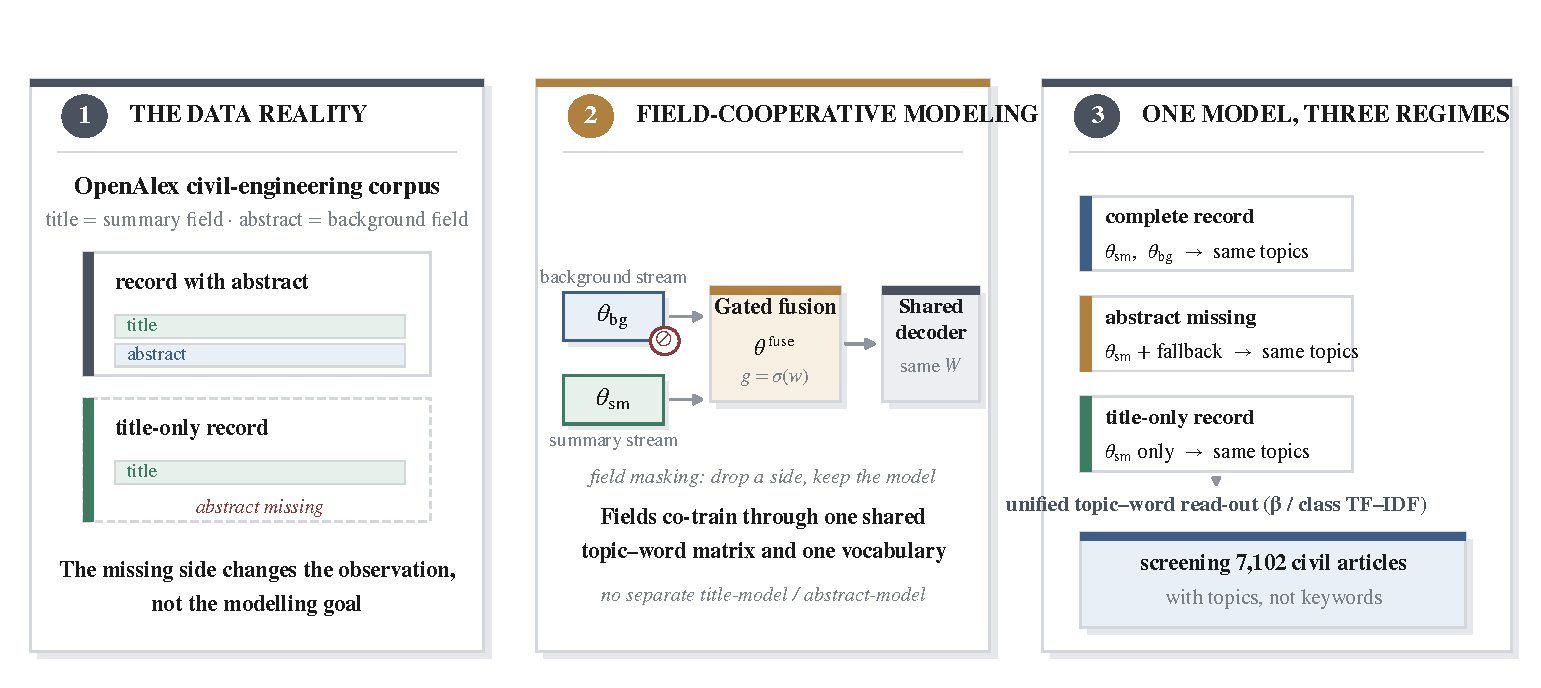
\includegraphics[width=0.98\linewidth]{Fig1.pdf}
\caption{Problem setting and contributions. (1) The application corpus is dual-field scholarly
metadata in which the abstract (background field) may be missing, leaving title-only records.
(2) \fcntm{} encodes both fields with separate conditional variational streams tied to one
shared topic--word decoder; field masking drops a side at training or inference time without
changing the model. (3) One trained model serves complete, abstract-missing and title-only
records through a unified topic--word read-out, supporting topic-based screening of
civil-engineering literature.}
\label{fig:concept}
\end{figure}

\section{Related work}
\label{sec:related}

\paragraph{Neural topic models.}
Neural topic models map a bag of words to a latent Gaussian posterior and decode topics from it:
NVDM applied variational auto-encoders to text \cite{miao2016nvdm}; AVITM develops autoencoding
variational inference, and its ProdLDA variant uses a linear decoder with a readable topic--word
matrix \cite{srivastava2017avitm}; CTM/CombinedTM concatenate sentence embeddings with counts
\cite{bianchi2021ctm}; and ETM defines topics in an embedding space \cite{dieng2020etm}. For
short texts, BTM models word pairs \cite{yan2013btm}; BERTopic uses class TF--IDF topic
representations \cite{grootendorst2022bertopic}, and Top2Vec learns joint document, word and
topic embeddings \cite{angelov2020top2vec}. GraphBTM and BCK-TM add word-pair structure
\cite{zhu2018graphbtm,zhang2020bcktm}, and BigARTM provides an additive regularisation framework
\cite{vorontsov2015bigartm}. Short-text neural topic modeling has also used topic-distribution
quantization with a negative-sampling decoder \cite{quantization2020}. Our decoder follows the
ProdLDA structure with topic orthogonality, dropout \cite{srivastava2014dropout} and
validation-based early stopping \cite{prechelt1998early}. The objectives, training loops and
learning rates differ across algorithms.

\paragraph{Multi-view, multimodal and structured-document models.}
Multi-view latent-variable learning and topic modelling share information across views:
multi-source variational inference \cite{kurle2019multisource}, robust multi-view topic modelling
\cite{zhang2017robust}, and disentangled or dual-view topic models
\cite{pergola2021disentangled,liu2022dualview}. Structured neural topic models for reviews
\cite{esmaeili2019structured} and metadata-conditioned models \cite{card2018metadata,roberts2019stm}
exploit additional document structure; CRNTM and DVI-DTM provide recent short-text examples
\cite{crntm2020,dvidtm2026}, alongside related word-pair models
\cite{relationalbtm2018,sparsebtm2021}. Kurle et al.\ encode each source separately and align
their posterior representations; JMVAE-kl infers a missing modality from the remaining one
\cite{suzuki2017jmvae}; and SubNTM models sub-document topics \cite{nguyen2026subntm}. Our
setting is fixed by the record schema: two textual fields share one vocabulary and one linear
decoder, and the study asks what field-restricted read-outs and missing-background inference
measure. The established components are applied to the field-level problem.

\paragraph{Text mining and topic modelling of engineering documents.}
Engineering informatics has an extensive text-mining literature on safety reports
\cite{civilsafety2015,civilaccident2018}, regulatory and contractual documents
\cite{compliance2013,ontology2015,contract2022,risknlp2023}, and domain surveys
\cite{civilnlp2021,civilnlp2023}. Topic models include DUET \cite{duet2019}, neural topic
modelling of building applications \cite{civiltopic2024} and passport taxonomies
\cite{passport2026}. These studies apply topic models to classification, thematic mapping and
taxonomy construction; the present study asks how fixed field structure affects field-restricted
read-out and missing-field inference.

\section{Methodology}
\label{sec:method}

Figure~\ref{fig:arch} gives an overview of \fcntm{}. The two fields are encoded by separate
conditional variational streams that share one topic decoder; the streams are tied by cross-field
reconstruction and a consistency term, and field-level masking with whole-field dropout covers
partially and fully missing fields.

\begin{figure}[!t]
\centering
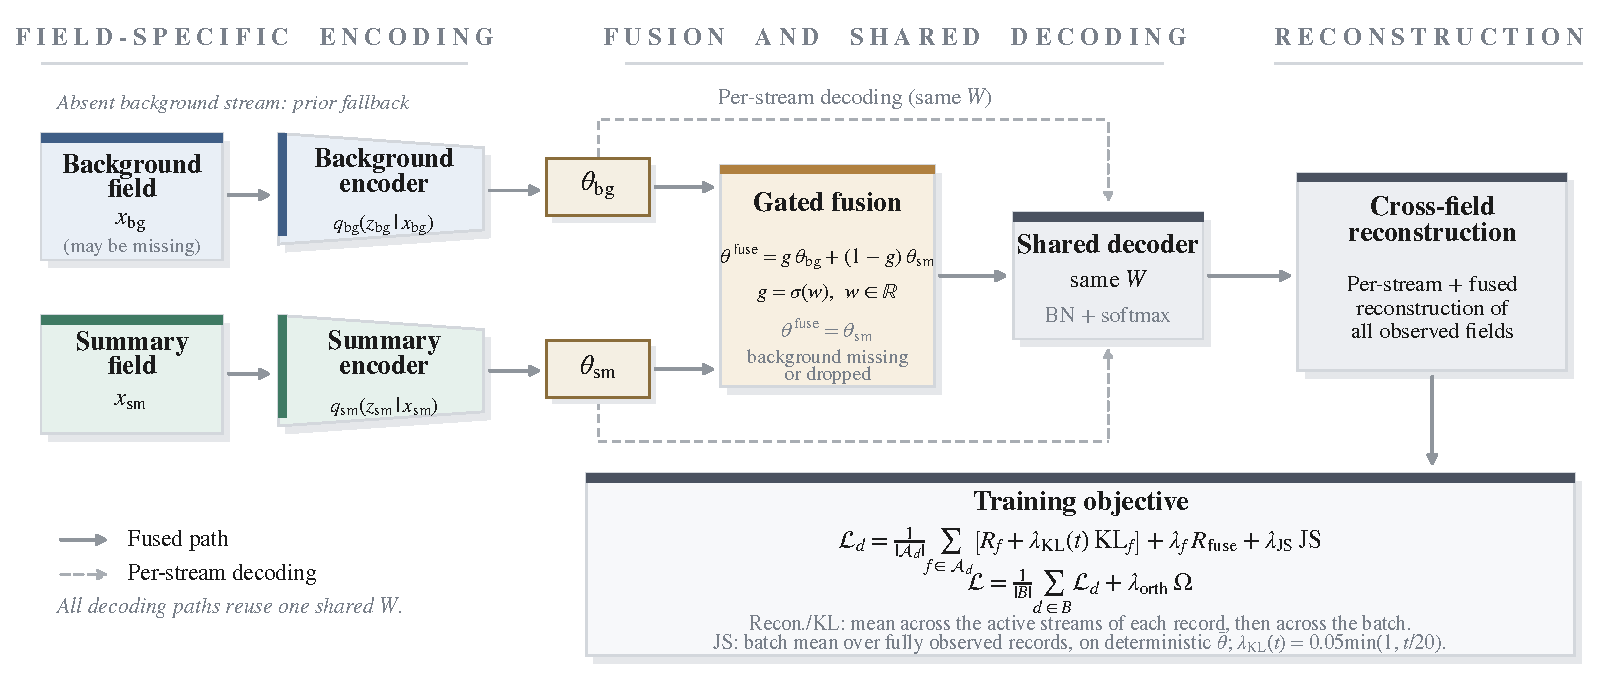
\includegraphics[width=0.98\linewidth]{Fig2.pdf}
\caption{Overview of \fcntm{}. Each field has its own conditional variational stream. Solid arrows
show the fused path, in which the gated mixture is decoded and every present field is reconstructed;
dashed arrows show the per-stream decodes, which reuse the same decoder parameters. The training
objective combines per-stream reconstruction, the KL terms of the active streams, fused
reconstruction, the JS term (computed only when both streams are active) and the topic-orthogonality
penalty. A missing or dropped field falls back to the prior, so the gated mixture reduces to the
remaining stream ($\theta^{\mathrm{fuse}}=\theta_{\mathrm{sm}}$ when the background field is missing
or dropped). The native $\beta$ read-out uses the raw matrix $W$, whereas generation follows the
batch-normalised path of Eq.~\eqref{eq:decode}.}
\label{fig:arch}
\end{figure}

\subsection{Problem setting}
Each record $d$ consists of field A (\emph{background}, e.g.\ the abstract of a paper or the body
of an issue) and field B (\emph{summary}, e.g.\ the title), with $N$ records in total and a shared
evaluation vocabulary of $V$ terms. The model maintains $K$ topics, a document--topic distribution
$\theta_d\in\Delta^{K-1}$, and a topic--word matrix $\beta\in\mathbb{R}^{K\times V}$ shared by both
fields. The task is to infer $\theta_d$ and $\beta$ from unlabelled records, to produce readable
topics in two read-outs, and to remain usable when one field is partially or entirely missing at
inference time.

\subsection{Field streams and the shared decoder}
Each field is encoded by its own two-layer MLP encoder (200 hidden units, Softplus activations,
dropout $0.2$) into the parameters of a field-conditioned Gaussian posterior,
\begin{equation}
q_f(z_f\mid x_f)=\mathcal N\big(\mu_f(x_f),\operatorname{diag}(\sigma_f^2(x_f))\big),
\qquad f\in\{\mathrm{bg},\mathrm{sm}\},
\label{eq:posterior}
\end{equation}
where $x_f$ is the $L_1$-normalised bag of words of field $f$ and $\log\sigma_f^2$ is capped at
$2$. Posterior means are mapped to topic proportions by a deterministic softmax,
$\bar\theta_f=\operatorname{softmax}(\mu_f(x_f))$, which is used at evaluation time in place of
sampling; $\bar\theta_f$ is a deterministic topic-proportion estimate and does not equal the
expectation of $\operatorname{softmax}(z_f)$. Both streams share one linear topic--word matrix
$W\in\mathbb{R}^{K\times V}$, and we write $\theta_f\in\mathbb{R}^{1\times K}$ for the topic
proportions of field $f$ under the row-vector convention,
\begin{equation}
p(w\mid\theta_f)=\operatorname{softmax}\!\big(\mathrm{BN}(\theta_f W)\big),
\label{eq:decode}
\end{equation}
where $\theta_f$ passes through dropout before the product, $\mathrm{BN}$ is a batch-normalisation
layer \emph{without} affine parameters applied over the vocabulary dimension (batch statistics
during training, running statistics at evaluation), and there is no additive bias. The $\beta$
read-out of Section~\ref{sec:readout} reads the raw rows of $W$, whereas generation uses the
normalised path of Eq.~\eqref{eq:decode}; the gap between the two is quantified in the
Supplementary Material.

\subsection{Training objective}
For a document $d$ let $\mathcal{G}_d$ collect its present fields (the background field is present
when the record carries it; the summary stream is always instantiated, including zero-vector
inputs after preprocessing) and let
$\mathcal{A}_d\subseteq\mathcal{G}_d$ be the \emph{active streams}, i.e.\ present fields whose
stream is not removed by whole-field dropout. Write $n^{(g)}_{dw}$ for the raw count of word $w$
in field $g$. Each active stream decodes once (Eq.~\eqref{eq:decode}) and reconstructs
\emph{every present field},
\begin{equation}
R_f=\sum_{g\in\mathcal{G}_d}\omega_g\,R_f(g),\qquad
R_f(g)=-\sum_{w=1}^{V} n^{(g)}_{dw}\,\log p\!\left(w\mid\theta_f\right),
\label{eq:recon}
\end{equation}
with fixed field weights $\omega_{\mathrm{bg}}=2.0$ and $\omega_{\mathrm{sm}}=1.0$. The summary
stream reconstructs the background field as well (cross-field reconstruction), and a background
field that was observed but dropped during training stays in the reconstruction targets even
though its own stream is inactive, whereas a naturally missing background field enters neither the
inputs nor the targets. The per-document objective is
\begin{equation}
\mathcal{L}_d=\frac{1}{|\mathcal{A}_d|}\sum_{f\in\mathcal{A}_d}
\Big[R_f+\lambda_{\mathrm{KL}}(t)\,\mathrm{KL}_f\Big]
+\lambda_f R_{\mathrm{fuse}}+\lambda_{\mathrm{JS}}\,\mathrm{JS},
\label{eq:total}
\end{equation}
where $\mathrm{KL}_f=\mathrm{KL}\big(q_f(z_f\mid x_f)\,\|\,\mathcal N(0,I)\big)$ is summed over
the $K$ latent dimensions and clamped at zero, and $\lambda_{\mathrm{KL}}(t)=0.05\min(1,t/20)$
anneals linearly during the first 20 epochs. The fused term
$R_{\mathrm{fuse}}=\sum_{g\in\mathcal{G}_d}\omega_g R_{\mathrm{fuse}}(g)$ is a second
reconstruction of both present fields from the fused topic mixture
\begin{equation}
\theta_d^{\mathrm{fuse}}=g\,\theta_{\mathrm{bg}}+(1-g)\,\theta_{\mathrm{sm}},
\qquad g=\sigma(w),\quad w\in\mathbb{R}.
\label{eq:lfuse}
\end{equation}
for records with both fields present, and
$\theta_d^{\mathrm{fuse}}=\theta_{\mathrm{sm}}$ when the background field is missing or
dropped. During training Eq.~\eqref{eq:lfuse} combines the \emph{sampled} per-stream
proportions that also feed the per-stream reconstructions; at inference time, and for the JS
term below, the deterministic estimates $\bar\theta_f$ are used. At inference,
Eq.~\eqref{eq:lfuse} is a convex combination of two deterministic topic-proportion estimates.
We refer to this quantity as a \emph{fused topic mixture} to distinguish it from a posterior. The
gate $g$ receives gradients only through $R_{\mathrm{fuse}}$, so with $\lambda_f=0$ the model
degenerates exactly to fixed mean fusion. The consistency term
\begin{equation}
\mathrm{JS}=\tfrac12\,\mathrm{KL}\!\big(\bar\theta_{\mathrm{bg}}\|m\big)
+\tfrac12\,\mathrm{KL}\!\big(\bar\theta_{\mathrm{sm}}\|m\big),
\qquad m=\tfrac12\big(\bar\theta_{\mathrm{bg}}+\bar\theta_{\mathrm{sm}}\big),
\label{eq:js}
\end{equation}
acts on the deterministic topic proportions and does not use the Gaussian posteriors. It is
computed only for documents whose two streams are both active and is not applied to records with
one active stream. A topic-orthogonality penalty keeps the rows of $W$ apart,
\begin{equation}
\Omega=\frac{1}{K(K-1)}\sum_{k\neq k'}\big|\cos\langle W_k,W_{k'}\rangle\big|,
\label{eq:orth}
\end{equation}
and the batch objective is $\frac{1}{|B|}\sum_{d\in B}\mathcal{L}_d
+\lambda_{\mathrm{orth}}\Omega$ with $\lambda_{\mathrm{orth}}=0.2$.

\subsection{Field masking}
Two masking mechanisms expose the model to missing fields, and they act on different units.
(i) \emph{Word-level input dropout} (denoising) is applied during training to the bag-of-words
\emph{word types} of each field: each bag-of-words dimension is independently zeroed with
probability $0.30$ (background) or $0.40$ (summary) in the encoder view only, while the
reconstruction targets remain the complete counts. (ii) \emph{Whole-field dropout} removes the
background stream of each training document with probability $0.5$ and substitutes the prior; the
summary stream is never dropped and learns to reconstruct both fields on its own. The test-time
occlusion protocol of Section~\ref{sec:occl} masks \emph{token positions} in the raw field text.
The training and evaluation procedures use different masking units. The consistency weight
$\lambda_{\mathrm{JS}}=0.5$, the fusion weight $\lambda_f=0.5$ and the dropout probabilities were
selected on held-out data.

\subsection{Optimisation}
Training uses Adam (learning rate $5\times10^{-4}$, momentum parameters $0.9$ and $0.999$),
mini-batches of $128$, gradient-norm clipping at $5.0$ and a budget of $700$ epochs. After the KL
warm-up the state with the lowest held-out loss is kept, for which $20\%$ of the training split is
held out; the patience is $150$ epochs. Evaluation-mode inference is deterministic: the
reparameterisation sampling is switched off and the held-out loss uses posterior means.
Numerical-anomaly recovery rolls the weights back to the most recent finite epoch, clears the
optimiser moments and halves the learning rate; this recovery step is separate from the
best-held-out-epoch selection of the early-stopping loop.

\subsection{Unified topic--word read-out}
\label{sec:readout}

Topic-word comparisons are only meaningful if every model is read out with the same vocabulary and
the same number of words per topic. We fix one evaluation vocabulary and exactly ten words per
topic. The \textbf{$\beta$ read-out} takes the top ten words of each normalised row of the model's
topic--word matrix; for \fcntm{} these are the raw rows of $W$, whereas generation uses
Eq.~\eqref{eq:decode}. LDA, BTM, NMF, ProdLDA, ETM, CTM-lite, CombinedTM and \fcntm{} are all
evaluated this way. The \textbf{class TF--IDF read-out} aggregates the training-term counts by the
soft document--topic assignment of the model, applies a BERTopic-style class TF--IDF transform
\cite{grootendorst2022bertopic}, and then takes the top ten words. Soft assignments replace the
hard cluster membership used in the standard class-level aggregation; for \fcntm{} this read-out
is built from the fused topic mixture $\bar\theta^{\mathrm{fuse}}$, which is why the two read-outs
can rank models differently. The sensitivity of the raw-parameter read-out relative to the
generative read-out is reported in the Supplementary Material.

\section{Experimental setup}
\label{sec:setup}

\subsection{Corpora and evaluation protocol}
We use three dual-field corpora. The \textbf{civil engineering corpus} is the application corpus:
title--abstract records of English-language scholarly works from OpenAlex \cite{openalex2022}
(\url{https://openalex.org}) in \emph{Civil and Structural Engineering} and \emph{Building and
Construction} (2000--2023; CC BY, CC BY-SA, or public-domain records). The sample comprises
7,102 articles, 889 conference papers and 9 reviews, split into 6000 training and 2000 test
records, with the title as the summary field and the abstract as the background field (mean
length ratio 11.2). \textbf{GitHub issues} \cite{openindex2026} pairs the issue body with its
title (four mature repositories, 6000/2000, ratio 12.9), and \textbf{AG News} \cite{zhang2015char}
pairs the description with the headline (6000/7600, ratio 3.9). All corpora are lower-cased and
tokenised on letter sequences; stop words and very short tokens are removed, the vocabulary is
built from the training split only, and test records never enter the vocabulary.
Table~\ref{tab:civil} reports the application corpus and Tables~\ref{tab:agnews} and~\ref{tab:github} report the two public corpora, all on the same evaluation vocabulary with exactly ten
words per topic and $K=30$. The evaluation protocol (vocabulary, ten words per topic, coherence
and diversity metrics) is shared by every model, whereas the training procedure differs across
algorithm families and is described in Section~\ref{sec:protocol}.
Because 400 records from each public test corpus were used during design, every public-corpus
result is also recomputed on a development-free subset (1600 GitHub and 7200 AG News records).
This rescoring excludes direct test overlap and is reported as a sensitivity analysis;
Section~\ref{sec:discussion} considers the remaining effect of prior model selection. The results
are organised around three questions: how well civil title--abstract records can be structured
into verifiable topics; how much signal remains when the abstract is missing; and how much the
complete field-cooperative configuration adds over a concatenated single-encoder control.
Cross-corpus diagnostics supplement these analyses.

\begin{table}[t]
\centering
\caption{Topic quality on AG News (unified evaluation vocabulary, ten words per topic; values are means over seeds 11/23/37 where applicable, and the training procedure differs across algorithm families as described in Section~\ref{sec:protocol}; BERTopic and Top2Vec choose their own topic numbers and are shown for reference).}
\label{tab:agnews}
\small
\begin{tabular}{lcccccc}
\toprule
Model & Topics & $C_V$ & NPMI & UMass & EXCL$_{\mathrm{KADJ}}$ & IRBO \\
\midrule
BTM & 30 & 0.600$\pm$0.011 & 0.164$\pm$0.005 & $-$4.19 & 0.409 & 0.980 \\
CombinedTM & 30 & 0.526$\pm$0.037 & 0.057$\pm$0.070 & $-$8.01 & 0.118 & 1.000 \\
\fcntm{}-cTFIDF & 30 & \textbf{0.612}$\pm$0.014 & \textbf{0.173}$\pm$0.012 & $-$4.20 & 0.193 & 0.974 \\
\fcntm{} & 30 & 0.586$\pm$0.026 & 0.137$\pm$0.022 & $-$4.91 & 0.013 & 0.993 \\
ETM & 30 & 0.506$\pm$0.014 & 0.092$\pm$0.010 & $-$5.12 & 0.439 & 0.982 \\
ProdLDA & 30 & 0.526$\pm$0.031 & 0.071$\pm$0.015 & $-$6.61 & 0.055 & 0.999 \\
Top2Vec & 2.7 & 0.498$\pm$0.032 & 0.099$\pm$0.031 & $-$2.92 & 0.268 & 0.937 \\
NMF & 30 & 0.494$\pm$0.015 & 0.069$\pm$0.013 & $-$5.96 & 0.799 & 0.997 \\
BERTopic & 29 & 0.488$\pm$0.022 & 0.035$\pm$0.026 & $-$8.81 & 0.681 & 0.997 \\
CTM-lite & 30 & 0.431$\pm$0.023 & $-$0.015$\pm$0.016 & $-$8.34 & 0.041 & 0.998 \\
LDA & 30 & 0.421$\pm$0.013 & $-$0.066$\pm$0.018 & $-$8.62 & 0.696 & 0.994 \\
\bottomrule
\end{tabular}
\end{table}

\begin{table}[t]
\centering
\caption{Topic quality on GitHub issues (same evaluation protocol and read-outs as Table~\ref{tab:agnews}; values are means over seeds 11/23/37; BERTopic and Top2Vec choose their own topic numbers and are shown for reference).}
\label{tab:github}
\small
\begin{tabular}{lcccccc}
\toprule
Model & Topics & $C_V$ & NPMI & UMass & EXCL$_{\mathrm{KADJ}}$ & IRBO \\
\midrule
BTM & 30 & 0.712$\pm$0.012 & 0.232$\pm$0.012 & $-$1.79 & 0.349 & 0.934 \\
\fcntm{}-cTFIDF & 30 & \textbf{0.727}$\pm$0.022 & \textbf{0.274}$\pm$0.026 & $-$1.90 & 0.133 & 0.901 \\
\fcntm{} & 30 & 0.701$\pm$0.016 & 0.233$\pm$0.012 & $-$3.16 & 0.010 & 0.967 \\
ETM & 30 & 0.675$\pm$0.014 & 0.213$\pm$0.010 & $-$2.14 & 0.366 & 0.955 \\
CombinedTM & 30 & 0.643$\pm$0.022 & 0.193$\pm$0.015 & $-$4.70 & 0.031 & 0.983 \\
NMF & 30 & 0.614$\pm$0.005 & 0.164$\pm$0.003 & $-$3.26 & 0.595 & 0.985 \\
ProdLDA & 30 & 0.579$\pm$0.007 & 0.107$\pm$0.012 & $-$5.21 & 0.043 & 0.995 \\
CTM-lite & 30 & 0.585$\pm$0.032 & 0.129$\pm$0.036 & $-$5.11 & 0.011 & 0.989 \\
LDA & 30 & 0.546$\pm$0.011 & 0.074$\pm$0.017 & $-$4.21 & 0.684 & 0.990 \\
BERTopic & 29 & 0.540$\pm$0.015 & 0.076$\pm$0.012 & $-$7.00 & 0.546 & 0.976 \\
Top2Vec & 160 & 0.493$\pm$0.009 & $-$0.008$\pm$0.013 & $-$9.65 & 0.337 & 0.994 \\
\bottomrule
\end{tabular}
\end{table}

\subsection{Baselines, training protocols and metrics}
\label{sec:protocol}

Baselines are LDA \cite{blei2003lda}, BTM \cite{yan2013btm}, NMF with a KL objective
\cite{lee2001nmf}, ProdLDA \cite{srivastava2017avitm}, ETM \cite{dieng2020etm}, CTM-lite, the
official CombinedTM \cite{bianchi2021ctm}, BERTopic \cite{grootendorst2022bertopic} and Top2Vec
\cite{angelov2020top2vec}; contextual models use Sentence-BERT embeddings \cite{reimers2019sbert}.
The implementations fall into four families with different training procedures: Gibbs sampling
(BTM, LDA), matrix factorisation (NMF), neural variational models (ProdLDA, ETM, CTM-lite and
\fcntm{} share the Adam loop \cite{kingma2015adam} and the 700-epoch budget but differ in learning
rate; the official CombinedTM keeps its own loop), and embedding clustering (BERTopic, Top2Vec),
which choose their own topic numbers and are shown for reference only. Full hyper-parameters are
listed in the Supplementary Material. Quality is measured by $C_V$ coherence
\cite{roder2015coherence}; NPMI \cite{bouma2009npmi,lau2014tea}; UCI and UMass
\cite{newman2010coherence,mimno2011coherence}; inter-topic diversity as one minus the mean
rank-biased overlap (RBO) with persistence $0.9$ and the residual tail retained for fixed
ten-word lists \cite{webber2010rbo}; and an exclusivity score based on Bischof and Airoldi
\cite{bischof2012exclusivity}, normalised by $K$ so that zero corresponds to the chance-level
value $1/K$. Topics with non-finite scores are dropped, so the effective topic count is recorded
next to every score.

\begin{table}[!t]
\centering
\caption{Topic quality on the civil engineering corpus (unified evaluation vocabulary, ten words
per topic; values are means over seeds 11/23/37, and the training procedure differs across
algorithm families as described in Section~\ref{sec:protocol}; BERTopic and Top2Vec choose their
own topic numbers and are shown for reference).}
\label{tab:civil}
\small
\begin{tabular}{lcccccc}
\toprule
Model & Topics & $C_V$ & NPMI & UMass & EXCL$_{\mathrm{KADJ}}$ & IRBO \\
\midrule
BTM & 30 & 0.583$\pm$0.010 & 0.128$\pm$0.009 & $-$2.18 & 0.283 & 0.944 \\
CombinedTM & 30 & 0.539$\pm$0.029 & 0.082$\pm$0.028 & $-$6.11 & 0.063 & 0.998 \\
\fcntm{}-cTFIDF & 30 & \textbf{0.636}$\pm$0.014 & \textbf{0.159}$\pm$0.011 & $-$2.21 & 0.165 & 0.937 \\
\fcntm{} & 30 & 0.633$\pm$0.014 & 0.154$\pm$0.022 & $-$2.85 & 0.014 & 0.990 \\
ETM & 30 & 0.581$\pm$0.012 & 0.119$\pm$0.007 & $-$2.75 & 0.379 & 0.963 \\
ProdLDA & 30 & 0.580$\pm$0.023 & 0.125$\pm$0.017 & $-$3.84 & 0.051 & 0.999 \\
Top2Vec & 153 & 0.515$\pm$0.002 & 0.029$\pm$0.011 & $-$8.52 & 0.359 & 0.995 \\
NMF & 30 & 0.598$\pm$0.009 & 0.135$\pm$0.006 & $-$2.86 & 0.559 & 0.984 \\
BERTopic & 29 & 0.576$\pm$0.026 & 0.116$\pm$0.027 & $-$5.06 & 0.563 & 0.991 \\
CTM-lite & 30 & 0.536$\pm$0.030 & 0.098$\pm$0.027 & $-$3.85 & 0.013 & 0.995 \\
LDA & 30 & 0.554$\pm$0.008 & 0.056$\pm$0.025 & $-$4.62 & 0.602 & 0.987 \\
\bottomrule
\end{tabular}
\end{table}

\section{Results and discussion}
\label{sec:results}

\subsection{Main results}
On the civil engineering corpus (Table~\ref{tab:civil}), \fcntm{} attains the highest coherence
among all evaluated models under both read-outs ($C_V=0.633$ for the $\beta$ read-out and $0.636$
for the class TF--IDF read-out; NPMI $0.154$ and $0.159$ over seeds 11/23/37), ahead of NMF
(0.598), BTM (0.583) and the neural baselines, and the ten-seed extension keeps both read-out
advantages (Table~\ref{tab:seed-paired}); Figure~\ref{fig:seedpaired} shows the per-seed
differences behind these means across all three corpora. Figure~\ref{fig:main} compares all evaluated models on the two public corpora under both coherence metrics.
On AG News, \fcntm{}-cTFIDF reaches $C_V=0.612$ and NPMI $=0.173$, above BTM under the matched
class TF--IDF read-out ($0.593$ / $0.169$) and above the $\beta$ read-outs of ProdLDA, ETM, NMF,
CTM-lite and LDA; under its own $\beta$ read-out BTM keeps a small lead ($0.600$ versus $0.586$).
On GitHub issues, \fcntm{}-cTFIDF reaches $C_V=0.727$ and NPMI $=0.274$, above BTM at both
read-outs ($0.712$ / $0.232$ for the native $\beta$ read-out, $0.700$ / $0.235$ matched), and
above the sentence-embedding baselines (CombinedTM $0.643$, BERTopic $0.540$).
The matched-read-out advantage over BTM is $+0.027$ $C_V$ and $+0.039$ NPMI on GitHub and
$+0.019$ / $+0.004$ on AG News for three seeds, but the per-seed structure differs: on GitHub all
three seeds are positive, whereas the AG News mean is carried by two of three seeds and the NPMI
advantage by one. On the development-free test subset the ordering is unchanged
(GitHub $0.734$ versus $0.711$, NPMI $0.284$ versus $0.248$; AG News $0.610$ versus $0.590$, NPMI
$0.172$ versus $0.167$; with BTM's native $\beta$ read-out, $0.734$ versus $0.726$ and $0.610$
versus $0.598$).

\begin{figure}[!t]
\centering
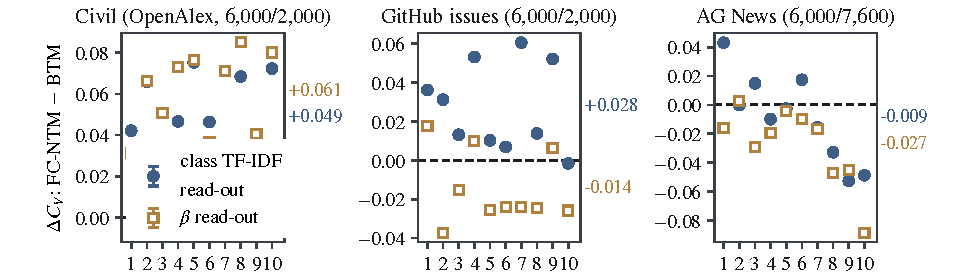
\includegraphics[width=0.98\linewidth]{Fig3.pdf}
\caption{Per-seed paired comparison of \fcntm{} and BTM (ten seeds per corpus, $C_V$). Each point
is one paired seed; the dashed line marks the BTM level. The class TF--IDF read-out is positive
in all ten paired seeds on the civil corpus and in nine of ten on GitHub issues, whereas the AG
News seeds are mixed. This is the corpus-dependent pattern that the mean differences summarise.}
\label{fig:seedpaired}
\end{figure}

\begin{figure}[t]
\centering
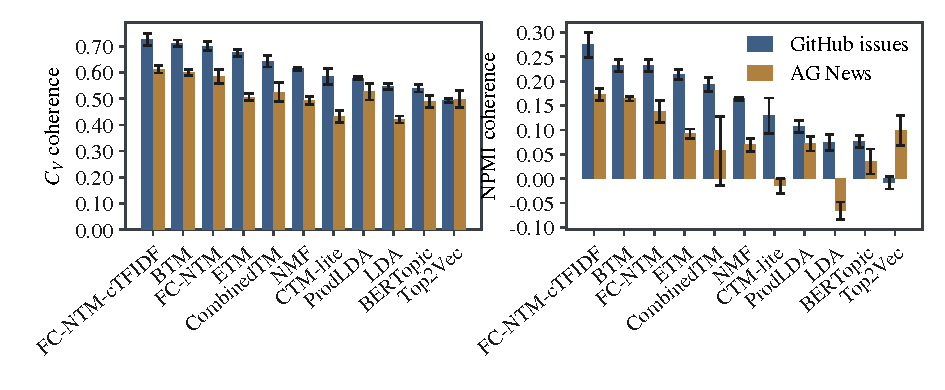
\includegraphics[width=0.86\textwidth]{Fig4.pdf}
\caption{Main results on the two public corpora (unified evaluation vocabulary, ten words per
topic). Left: $C_V$; right: NPMI. Error bars are standard deviations across seeds 11/23/37.}
\label{fig:main}
\end{figure}

\subsection{Read-out-matched comparison}
Table~\ref{tab:fair} collects the read-out-matched comparison across models and read-outs.

The class TF--IDF read-out depends on the model and the corpus: on GitHub it lifts CTM-lite,
ProdLDA and LDA by $0.091$, $0.087$ and $0.068$ but leaves ETM and NMF unchanged or worse, while
on AG News it helps every model except BTM. Comparisons use the matched read-out. Under it,
\fcntm{}-cTFIDF leads the strongest GitHub baselines (BTM $0.700$, CTM-lite $0.675$, ETM $0.669$,
ProdLDA $0.666$) by $0.027$--$0.061$ $C_V$ and $0.039$--$0.059$ NPMI, larger than its
seed-to-seed standard deviation ($0.022$); on AG News the advantage over BTM is $+0.019$ $C_V$
but rests on two of three seeds; under the native $\beta$ read-out the AG News means are $0.586$
for \fcntm{} and $0.600$ for BTM. On the civil corpus NMF ($0.607$) and ETM ($0.603$) exceed BTM
($0.590$), and \fcntm{}-cTFIDF leads them by $0.029$ and $0.033$ $C_V$, although the ten-seed
comparison is against BTM. Figure~\ref{fig:heatmap} visualises the same comparison; within each
panel one colour scale spans all corpora and read-outs, the boxed first row is \fcntm{}, and
bold entries mark the best model per column.

\begin{figure}[!t]
\centering
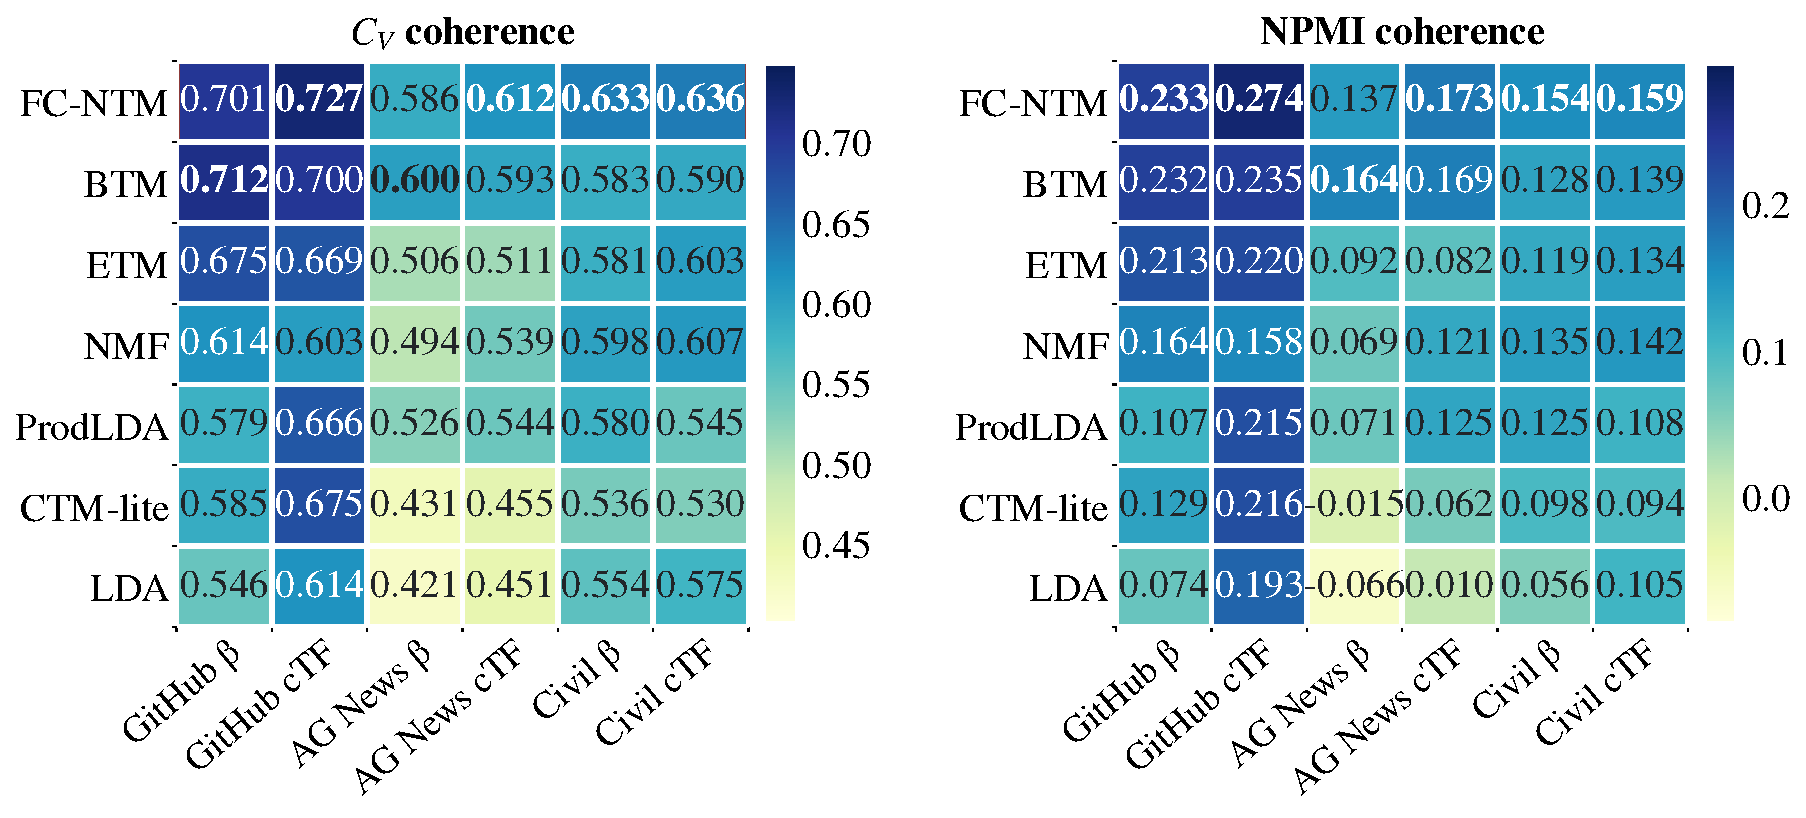
\includegraphics[width=0.98\linewidth]{Fig5.pdf}
\caption{The read-out comparison of Table~\ref{tab:fair} as a heatmap ($K=30$, means over seeds
11/23/37). Left: $C_V$; right: NPMI. Columns combine the three corpora with the two read-outs
(native $\beta$; class TF--IDF). The boxed first row is \fcntm{}; bold entries mark the
column-wise best.}
\label{fig:heatmap}
\end{figure}

\begin{table}[t]
\centering
\caption{Read-out comparison ($K=30$, means over seeds 11/23/37). Each model is first read out through its own topic--word matrix ($\beta$ read-out) and then through a class TF--IDF read-out aggregated from its training-set posterior $\theta$; BTM enters the same read-out through the point-estimate document--topic posterior of its original Section 3.3, and the FC-NTM row is the same model as in Tables~\ref{tab:agnews} and~\ref{tab:github}.}
\label{tab:fair}
\footnotesize
\setlength{\tabcolsep}{4pt}
\begin{tabular}{@{}llcc@{}}
\toprule
Corpus & Model & $\beta$ read-out $C_V$ / NPMI & Class TF--IDF $C_V$ / NPMI \\
\midrule
 \multirow{7}{*}{GitHub}
 & \fcntm{}(3 seed mean) & 0.701 / 0.233 & \textbf{0.727 / 0.274} \\
 & ETM & 0.675 / 0.213 & 0.669 / 0.220 \\
 & ProdLDA & 0.579 / 0.107 & 0.666 / 0.215 \\
 & CTM-lite & 0.585 / 0.129 & 0.675 / 0.216 \\
 & NMF & 0.614 / 0.164 & 0.603 / 0.158 \\
 & LDA & 0.546 / 0.074 & 0.614 / 0.193 \\
 & BTM(3 seeds) & 0.712 / 0.232 & 0.700 / 0.235 \\
\midrule
 \multirow{7}{*}{AG News}
 & \fcntm{}(3 seed mean) & 0.586 / 0.137 & \textbf{0.612 / 0.173} \\
 & ProdLDA & 0.526 / 0.071 & 0.544 / 0.125 \\
 & NMF & 0.494 / 0.069 & 0.539 / 0.121 \\
 & ETM & 0.506 / 0.092 & 0.511 / 0.082 \\
 & CTM-lite & 0.431 / $-$0.015 & 0.455 / 0.062 \\
 & LDA & 0.421 / $-$0.066 & 0.451 / 0.010 \\
 & BTM(3 seeds) & 0.600 / 0.164 & 0.593 / 0.169 \\
\midrule
 \multirow{7}{*}{Civil corpus}
 & \fcntm{}(3 seed mean) & \textbf{0.633 / 0.154} & \textbf{0.636 / 0.159} \\
 & NMF & 0.598 / 0.135 & 0.607 / 0.142 \\
 & ETM & 0.581 / 0.119 & 0.603 / 0.134 \\
 & BTM(3 seeds) & 0.583 / 0.128 & 0.590 / 0.139 \\
 & LDA & 0.554 / 0.056 & 0.575 / 0.105 \\
 & ProdLDA & 0.580 / 0.125 & 0.545 / 0.108 \\
 & CTM-lite & 0.536 / 0.098 & 0.530 / 0.094 \\
\bottomrule
\end{tabular}
\end{table}

\subsection{Ten-seed paired comparison}
To test whether the three-seed differences are seed noise, we extend \fcntm{} and BTM to ten
seeds on all three corpora (adding 53/71/89/101/113/127/139) and compare both read-outs and the
occlusion behaviour seed by seed. Occlusion comparisons are limited to preselected baselines:
BTM on all three corpora and LDA additionally on AG News.

\begin{table}[!t]
\centering
\caption{Ten-seed paired comparison of \fcntm{} and BTM on the three corpora. The read-out rows
report $C_V$ differences (\fcntm{} minus BTM at the same read-out); the occlusion rows compare
the relative degradation $\mathrm{NLL}(100\%)/\mathrm{NLL}(25\%)$, so a positive value means
\fcntm{} is more stable. Occlusion comparisons are limited to preselected baselines: BTM on all
three corpora and LDA additionally on AG News. CIs are two-sided 95\% $t$ intervals; sign and
Wilcoxon tests are two-sided.}
\label{tab:seed-paired}
\footnotesize
\setlength{\tabcolsep}{4pt}
\begin{tabular}{@{}llcccccc@{}}
\toprule
Corpus & Comparison & Mean diff. & CI low & CI high & Positive & Sign $p$ & Wilcoxon $p$ \\
\midrule
GitHub & Class TF--IDF & $+$0.028 & $+$0.012 & $+$0.043 & 9/10 & 0.021 & 0.004 \\
GitHub & $\beta$ read-out & $-$0.014 & $-$0.028 & $-$0.001 & 3/10 & 0.344 & 0.037 \\
GitHub & Occlusion (vs.\ BTM) & $+$0.024 & $+$0.022 & $+$0.026 & 10/10 & 0.002 & 0.002 \\
\midrule
AG News & Class TF--IDF & $-$0.009 & $-$0.030 & $+$0.013 & 3/10 & 0.344 & 0.375 \\
AG News & $\beta$ read-out & $-$0.027 & $-$0.047 & $-$0.008 & 1/10 & 0.021 & 0.004 \\
AG News & Occlusion (vs.\ BTM) & $+$0.025 & $+$0.024 & $+$0.026 & 10/10 & 0.002 & 0.002 \\
AG News & Occlusion (vs.\ LDA) & $-$0.013 & $-$0.014 & $-$0.012 & 0/10 & 0.002 & 0.002 \\
\midrule
Civil corpus & Class TF--IDF & $+$0.049 & $+$0.033 & $+$0.064 & 10/10 & 0.002 & 0.002 \\
Civil corpus & $\beta$ read-out & $+$0.061 & $+$0.047 & $+$0.075 & 10/10 & 0.002 & 0.002 \\
Civil corpus & Occlusion (vs.\ BTM) & $-$0.003 & $-$0.004 & $-$0.002 & 0/10 & 0.002 & 0.002 \\
\bottomrule
\end{tabular}
\end{table}

For GitHub, the class TF--IDF difference is $+0.028$ $C_V$ (95\% CI $[+0.012,+0.043]$, 9/10
positive seeds), and the relative-degradation difference is $+0.024$ (10/10). On the civil
corpus, the class TF--IDF and native $\beta$ differences are $+0.049$ and $+0.061$ $C_V$, with
10/10 positive paired differences; the occlusion difference is $-0.003$ (0/10). On AG News, the
class TF--IDF difference is $-0.009$ (95\% CI $[-0.030,+0.013]$, 3/10) and the native $\beta$
difference is $-0.027$ (1/10). The native $\beta$ difference on GitHub is $-0.014$ (3/10). The
class TF--IDF mean differences across the three corpora are $+0.049$, $+0.028$ and $-0.009$.
Confidence intervals describe training and masking randomness under a fixed corpus and design.

\subsection{Field redundancy and the gain}
Table~\ref{tab:conditional} reports the held-out redundancy measures together with the observed gains, and Figure~\ref{fig:cond} relates them across the two public corpora.

The redundancy measures are fitted on the training split and evaluated on the test split for the
two public corpora. Their held-out predictability is 0.306 for GitHub and 0.245 for AG News
($\rho^2_{\mathrm{cca}}$). At three seeds, the matched class TF--IDF differences from BTM are
$+0.027$ and $+0.019$; the ten-seed differences are $+0.028$ (9/10) and $-0.009$ (3/10). The
corresponding civil difference is $+0.049$ (10/10), as reported in Table~\ref{tab:seed-paired}.
Whole-field occlusion changes coherence by $+0.009\pm0.022$ on GitHub and $+0.018\pm0.013$ on
AG News.

\begin{table}[t]
\centering
\caption{Field redundancy, measured occlusion gap and the $C_V$ difference against BTM on two corpora. Redundancy is fitted on the training split and evaluated on the test split and includes constructive controls (exact copy $=1.000$, cross-document shuffle $\approx0.000$); the occlusion $\Delta C_V$ is the mean$\pm$standard deviation over seeds 11/23/37 with dropout training. The last column gives the $C_V$ difference under the matched class TF--IDF read-out and under BTM's native $\beta$ read-out.}
\label{tab:conditional}
\footnotesize
\setlength{\tabcolsep}{4pt}
\begin{tabular}{@{}lcccc@{}}
\toprule
Corpus & Held-out Ridge $R^2$ & Held-out $\rho^2_{\mathrm{cca}}$
 & Occlusion $\Delta C_V$ & $C_V$ gap, cTFIDF$-$BTM (matched / $\beta$) \\
\midrule
GitHub issues & 0.230 & 0.306 & $+$0.009$\pm$0.022 & $+$0.027 / $+$0.014 \\
AG News & 0.158 & 0.245 & $+$0.018$\pm$0.013 & $+$0.019 / $+$0.012 \\
\bottomrule
\end{tabular}
\end{table}

\begin{figure}[t]
\centering
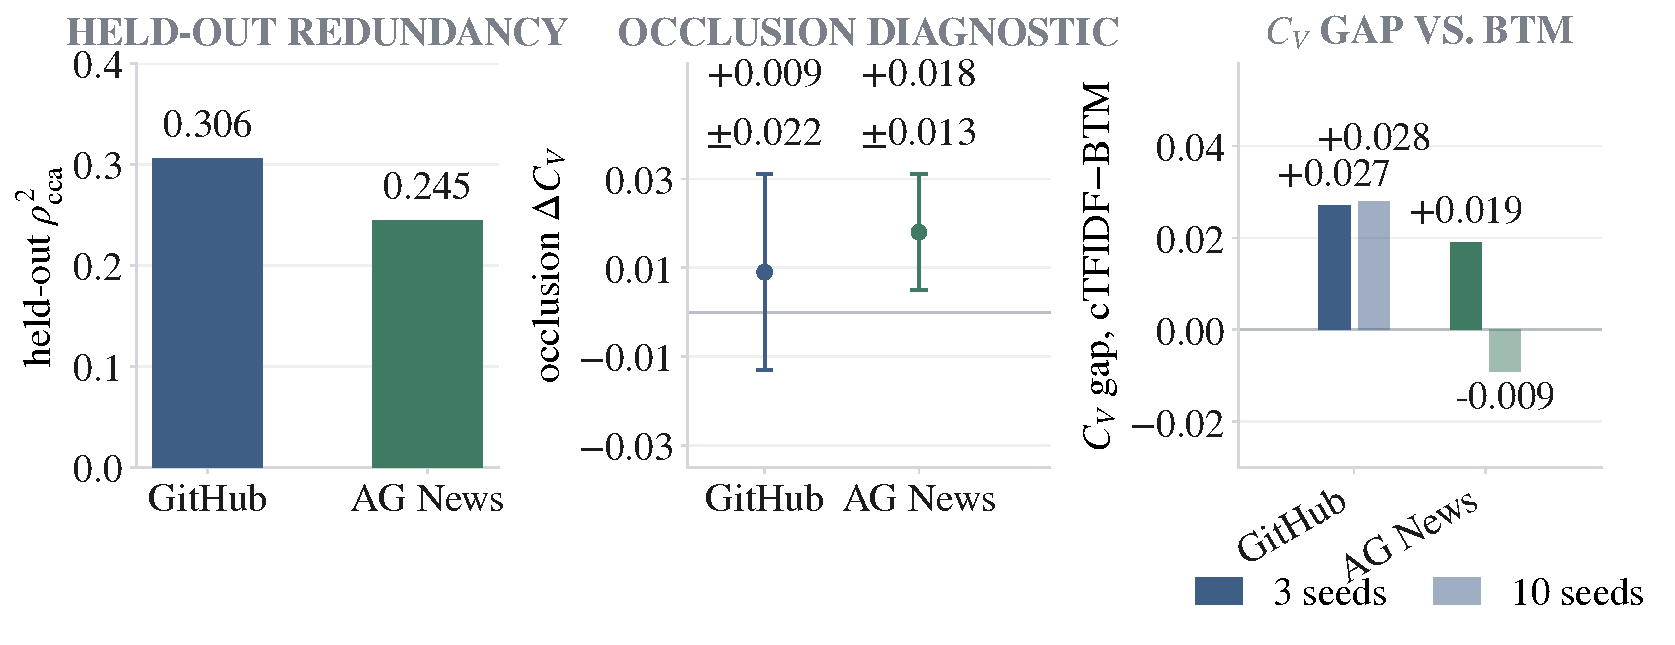
\includegraphics[width=0.86\textwidth]{Fig6.pdf}
\caption{Field redundancy and gain (held-out measures). Left: squared canonical correlation $\rho^2_{\mathrm{cca}}$ (higher means more redundant), fitted on the training split and evaluated on the test split. Middle: occlusion diagnostic $\Delta C_V$ (mean$\pm$standard deviation over seeds 11/23/37). Right: the $C_V$ difference of \fcntm{}-cTFIDF against BTM under the matched class TF--IDF read-out (three seeds) and the ten-seed paired difference. The two corpora reach similar held-out redundancy, while the ten-seed difference is $+0.028$ on GitHub and $-0.009$ on AG News.}\label{fig:cond}
\end{figure}

\subsection{Field inference under partial occlusion}
\label{sec:occl}

A direct test of field complementarity is whether the visible field B helps a model recover
content when part of field A is unavailable. The protocol (Supplementary Material) masks a
fraction $p$ of the background-field tokens in the test documents, re-infers the topic
proportions from the remaining input, and scores the occluded tokens under the model's own word
distribution; it reports the per-token negative log-likelihood (NLL), the agreement of the most
probable topic with the unoccluded inference, and the posterior JS divergence. Every model uses
its own inference path and its own word distribution, so no cross-model read-out convention is
involved. When a document has no visible evidence at all, BTM and NMF use the training-corpus
topic prior; treating a zero vector as a word distribution would inflate the NLL to
$\log 10^{12}=27.63$. Table~\ref{tab:occl-robust} reports the per-condition values on GitHub issues, and Figure~\ref{fig:occlusion} plots the NLL and relative-degradation curves
behind them.

From 25\% to 100\% occlusion the per-token NLL of \fcntm{} rises by only 3.2\%
($7.712\to7.960$), less than LDA (7.4\%), ProdLDA (8.0\%), ETM (8.9\%), BTM (5.2\%) and NMF
(47.1\%), which is consistent with the training-time whole-field dropout. At full occlusion, BTM
has the lowest NLL (6.972); topic agreement is highest for NMF (0.469), followed by ETM (0.452),
while \fcntm{} reaches 0.358. We report relative degradation together with absolute NLL and
agreement, which provide calibration and input-sensitivity information. The protocol covers
three English corpora with ten seeds per corpus, with occlusion masks redrawn for each seed,
and the field split follows existing title/body structure.

\begin{figure}[!t]
\centering
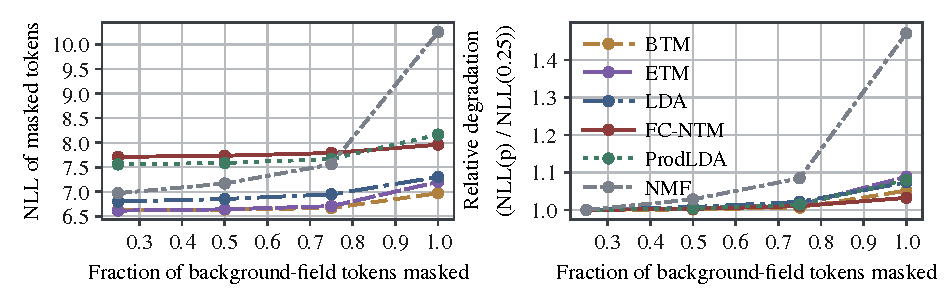
\includegraphics[width=0.86\linewidth]{Fig7.pdf}
\caption{Inference behaviour under partial occlusion of the background field (GitHub issues,
seed 11, 2000 test documents). Left: per-token negative log-likelihood of the occluded tokens;
right: relative degradation $\mathrm{NLL}(p)/\mathrm{NLL}(0.25)$, which summarises the relative
increase from the 25\% condition. \fcntm{} is trained with whole-field dropout at $p=0.5$ and has
the smallest relative degradation ($\times1.032$). The figure also reports absolute NLL to
contextualise this ratio; topic agreement is reported in Table~\ref{tab:occl-robust}.}
\label{fig:occlusion}
\end{figure}

\begin{table}[t]
\centering
\caption{Partial-occlusion curves on GitHub issues (seed 11). NLL is the per-token negative log-likelihood of the occluded tokens (lower is better); relative degradation is $\mathrm{NLL}(100\%)/\mathrm{NLL}(25\%)$; agreement is the fraction of documents holding their most probable topic at 100\% occlusion. BTM enters through its document--topic posterior.}
\label{tab:occl-robust}
\footnotesize
\setlength{\tabcolsep}{3pt}
\begin{tabular}{@{}lccccc@{}}
\toprule
Model & NLL(25\%) & NLL(50\%) & NLL(75\%) & NLL(100\%) & Degradation / Agreement \\
\midrule
\fcntm{} & 7.712 & 7.735 & 7.790 & 7.960 & \textbf{1.032} / 0.358 \\
LDA & 6.802 & 6.854 & 6.948 & 7.302 & 1.074 / 0.420 \\
ProdLDA & 7.558 & 7.588 & 7.668 & 8.165 & 1.080 / 0.354 \\
BTM & 6.630 & 6.639 & 6.670 & \textbf{6.972} & 1.052 / 0.448 \\
ETM & \textbf{6.616} & 6.643 & 6.708 & 7.202 & 1.089 / 0.452 \\
NMF & 6.972 & 7.169 & 7.561 & 10.255 & 1.471 / \textbf{0.469} \\
\bottomrule
\end{tabular}
\end{table}

\subsection{Cross-corpus comparison}
Table~\ref{tab:occl-cross} and Figure~\ref{fig:occl-cross} extend the same protocol to the three corpora.

On GitHub (ratio 12.9), all models degrade by factors of $\times1.028$--$\times1.467$, and
\fcntm{} has the smallest relative degradation; the ten-seed paired difference from BTM is
$+0.024\pm0.004$ (10/10). On the civil corpus (ratio 11.2), the relative degradations are 1.010
for \fcntm{} and 1.007 for BTM (paired difference $-0.003$, 0/10). On AG News (ratio 3.9), they
are 1.019 for \fcntm{} and 1.006 for LDA. Held-out mutual prediction is slightly higher for
GitHub, while the length ratio and background-exclusive share distinguish GitHub from AG News and
place the civil corpus in a similar range to GitHub. These statistics serve as corpus descriptors
for the three evaluated collections.

\begin{table}[t]
\centering
\caption{Partial-occlusion behaviour on the three corpora (ten seeds 11--139, mean$\pm$standard deviation; the mask is redrawn per seed). Bold marks the smallest relative degradation per corpus. Field asymmetry is described by the mean background/summary token ratio and by the token-type share of background words that do not occur in the summary of the same document.}
\label{tab:occl-cross}
\footnotesize
\setlength{\tabcolsep}{3pt}
\begin{tabular}{@{}llcc@{}}
\toprule
Corpus(Field asymmetry) & Model & Relative degradation & Agreement(100\%) \\
\midrule
\multirow{6}{*}{\shortstack[l]{GitHub issues\\ Length ratio 12.9\\ Background-exclusive 0.877}}
 & \fcntm{} & \textbf{1.028$\pm$0.003} & 0.364 \\
 & LDA & 1.075$\pm$0.003 & 0.416 \\
 & ProdLDA & 1.078$\pm$0.004 & 0.343 \\
 & ETM & 1.087$\pm$0.003 & 0.451 \\
 & BTM & 1.052$\pm$0.001 & 0.443 \\
 & NMF & 1.467$\pm$0.009 & 0.464 \\
\midrule
\multirow{6}{*}{\shortstack[l]{Civil corpus\\ Length ratio 11.2\\ Background-exclusive 0.894}}
 & \fcntm{} & 1.010$\pm$0.001 & 0.661 \\
 & LDA & 1.037$\pm$0.002 & 0.574 \\
 & ProdLDA & 1.028$\pm$0.002 & 0.558 \\
 & ETM & 1.041$\pm$0.001 & 0.656 \\
 & BTM & \textbf{1.007$\pm$0.001} & 0.565 \\
 & NMF & 1.172$\pm$0.002 & 0.651 \\
\midrule
\multirow{6}{*}{\shortstack[l]{AG News\\ Length ratio 3.9\\ Background-exclusive 0.868}}
 & \fcntm{} & 1.019$\pm$0.001 & 0.515 \\
 & LDA & \textbf{1.006$\pm$0.002} & 0.440 \\
 & ProdLDA & 1.026$\pm$0.001 & 0.491 \\
 & ETM & 1.072$\pm$0.002 & 0.561 \\
 & BTM & 1.044$\pm$0.001 & 0.553 \\
 & NMF & 1.411$\pm$0.004 & 0.545 \\
\bottomrule
\end{tabular}
\end{table}

\begin{figure}[t]
\centering
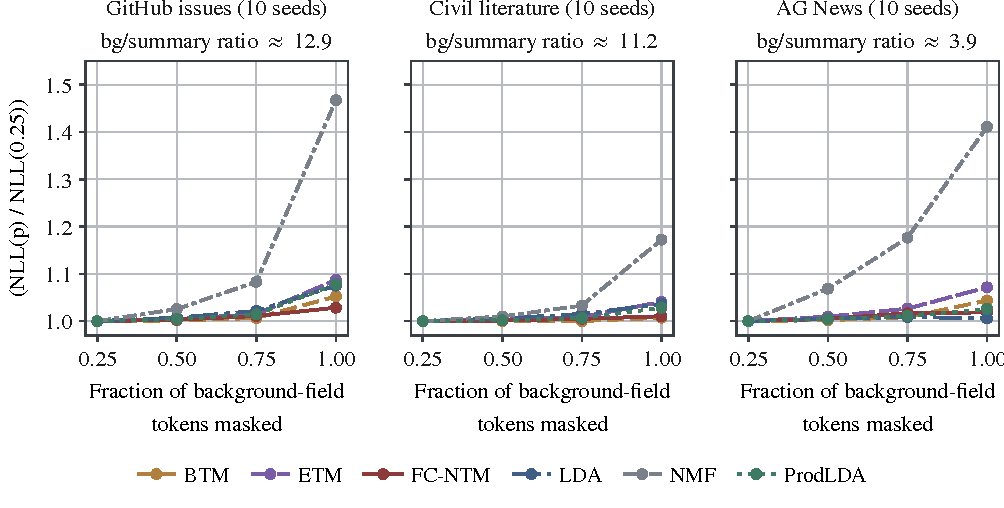
\includegraphics[width=0.86\textwidth]{Fig8.pdf}
\caption{Relative degradation under the same partial-occlusion protocol on three corpora (curves
are means, shading is $\pm1$ standard deviation; all six models cover the ten seeds 11--139).
Left: GitHub issues
(background to summary length ratio $\approx12.9$); middle: civil engineering corpus
($\approx11.2$); right: AG News ($\approx3.9$). Only on GitHub is the degradation of \fcntm{}
below all baselines; on the civil corpus and AG News the smallest degradation belongs to
BTM and LDA respectively, and the gap to \fcntm{} is within 0.003--0.013.}
\label{fig:occl-cross}
\end{figure}
\subsection{Field-restricted read-out}

\begin{table}[t]
\centering
\caption{Field-restricted read-out ($C_V$, mean$\pm$standard deviation over seeds 11/23/37). Every topic--word matrix is truncated to the vocabulary of one field and scored against that field's test text only; ``background view'' is the abstract/body side and ``summary view'' the title side. FC-NTM's summary view is scored on 20--22 scorable topics per seed on GitHub (29--30 on AG News, 26--28 on the civil corpus) because topics whose ten field words never occur in the held-out text get an undefined $C_V$.}
\label{tab:fieldview-baselines}
\small
\setlength{\tabcolsep}{4pt}
\begin{tabular}{@{}llcc@{}}
\toprule
Corpus & Model & Background view $C_V$ & Summary view $C_V$ \\
\midrule
\multirow{5}{*}{GitHub issues}
 & \fcntm{} & 0.697$\pm$0.016 & 0.426$\pm$0.012 \\
 & BTM & \textbf{0.710$\pm$0.011} & 0.396$\pm$0.018 \\
 & NMF & 0.609$\pm$0.004 & 0.433$\pm$0.002 \\
 & LDA & 0.543$\pm$0.011 & 0.466$\pm$0.005 \\
 & ProdLDA & 0.575$\pm$0.006 & \textbf{0.467$\pm$0.034} \\
\midrule
\multirow{5}{*}{AG News}
 & \fcntm{} & 0.566$\pm$0.016 & 0.423$\pm$0.015 \\
 & BTM & \textbf{0.586$\pm$0.015} & 0.399$\pm$0.018 \\
 & NMF & 0.477$\pm$0.015 & 0.444$\pm$0.002 \\
 & LDA & 0.419$\pm$0.007 & \textbf{0.486$\pm$0.006} \\
 & ProdLDA & 0.499$\pm$0.032 & 0.438$\pm$0.007 \\
\midrule
\multirow{5}{*}{Civil corpus}
 & \fcntm{} & \textbf{0.637$\pm$0.015} & 0.408$\pm$0.005 \\
 & BTM & 0.589$\pm$0.014 & 0.382$\pm$0.008 \\
 & NMF & 0.600$\pm$0.009 & 0.398$\pm$0.013 \\
 & LDA & 0.554$\pm$0.008 & 0.415$\pm$0.006 \\
 & ProdLDA & 0.576$\pm$0.025 & \textbf{0.419$\pm$0.012} \\
\bottomrule
\end{tabular}
\end{table}

Field-restricted read-out truncates the topic words to one field's vocabulary and scores them
against that field's own test text. With the shared decoder, the background-view $C_V$ of
\fcntm{} stays close to its full-vocabulary $\beta$ read-out on all three corpora (0.697, 0.566
and 0.637 versus 0.701, 0.586 and 0.633), while the summary view is lower in absolute terms mainly
because a summary contains only 3--5 tokens and the reference corpus is very short, so that column
should be compared within the same protocol. The cross-model comparison shows that the
read-out is not unique to a two-stream encoder: BTM is slightly better in the background view on
GitHub and AG News (0.710 versus 0.697 and 0.586 versus 0.566), \fcntm{} leads on the civil
corpus (0.637 versus 0.600 for NMF), and in the summary view LDA and ProdLDA are above \fcntm{}
on all three corpora (0.486 and 0.438 versus 0.423 on AG News). The field view thus serves as a
descriptive read-out available to any model with a topic--word matrix.

\subsection{Ablation: fusion reconstruction and gating}

\begin{table}[t]
\centering
\caption{Three-step fusion ablation on GitHub issues ($K=30$, seeds 11/23/37, same protocol). Within one read-out each row changes exactly one thing: first the fused mixture $\theta_{\mathrm{fuse}}$ is decoded into the reconstruction term (mean fusion), then mean fusion is replaced by a learnable gate (the main model). ``Positive pairs'' counts the seeds whose paired difference against the row above is positive ($C_V$, NPMI).}
\label{tab:fusion}
\small
\begin{tabular}{llcccc}
\toprule
Read-out & Configuration & $C_V$ & NPMI & Positive pairs & UMass \\
\midrule
\multirow{3}{*}{$\beta$} & No fusion & 0.721$\pm$0.016 & 0.266$\pm$0.012 & --- & $-$2.63 \\
 & Mean fusion + fusion recon. & 0.708$\pm$0.016 & 0.245$\pm$0.013 & 1/3, 0/3 & $-$2.98 \\
 & Gated fusion (main model) & 0.701$\pm$0.016 & 0.233$\pm$0.012 & 0/3, 0/3 & $-$3.16 \\
\midrule
\multirow{3}{*}{cTFIDF} & No fusion & 0.714$\pm$0.001 & 0.262$\pm$0.007 & --- & $-$1.86 \\
 & Mean fusion + fusion recon. & 0.728$\pm$0.007 & 0.275$\pm$0.015 & 3/3, 3/3 & $-$1.91 \\
 & Gated fusion (main model) & 0.727$\pm$0.022 & 0.274$\pm$0.026 & 1/3, 1/3 & $-$1.90 \\
\bottomrule
\end{tabular}
\end{table}

The three-step ablation separates two questions: whether the fused mixture receives its own
reconstruction term, and whether fusion is averaged or gated. The fusion-reconstruction term is
effective, but only for the read-out that uses the fused posterior: adding it under mean fusion
raises the class TF--IDF $C_V$ and NPMI by 0.014 and 0.013 (3/3 seeds) while lowering the $\beta$
read-out by 0.013 and 0.021. Replacing mean fusion by a gate brings no further gain in this corpus
and protocol (class TF--IDF differences $-0.001$ and $-0.000$, 1/3 seeds; $\beta$ read-out
$-0.007$ and $-0.012$, 0/3): within this corpus and protocol, the gate adds no gain over mean
fusion once the fusion-reconstruction term is present.

\subsection{Ablation: core components}

\begin{table}[t]
\centering
\caption{Core-component ablation on three corpora and two read-outs ($K=30$, seeds 11/23/37, 700-epoch budget, all other settings identical to the main model). Each column switches off one component: cross-field reconstruction of both streams, the JS consistency weight, field-level word masking, and whole-field dropout; the fusion-reconstruction term is kept in all columns. Values are mean paired $\Delta C_V$ (negative means the component matters), parentheses count positive pairs.}
\label{tab:core-ablation}
\small
\setlength{\tabcolsep}{5pt}
\begin{tabular}{llcccc}
\toprule
Corpus & Read-out & $-$Cross-field recon. & $-$JS consistency & $-$Word masking & $-$Field dropout \\
\midrule
GitHub & $\beta$ & $+$0.021 (2/3) & $-$0.001 (1/3) & $-$0.012 (1/3) & $-$0.023 (1/3) \\
GitHub & Class TF-IDF & $-$0.005 (1/3) & $+$0.004 (2/3) & $-$0.004 (1/3) & $-$0.021 (1/3) \\
\midrule
AG News & $\beta$ & $-$0.011 (2/3) & $+$0.003 (1/3) & $-$0.026 (0/3) & $-$0.010 (1/3) \\
AG News & Class TF-IDF & $-$0.022 (0/3) & $-$0.002 (1/3) & $-$0.043 (0/3) & $-$0.023 (1/3) \\
\midrule
Civil corpus & $\beta$ & $-$0.022 (0/3) & $+$0.001 (2/3) & $-$0.010 (1/3) & $+$0.001 (1/3) \\
Civil corpus & Class TF-IDF & $-$0.019 (0/3) & $-$0.002 (0/3) & $-$0.012 (0/3) & $-$0.034 (0/3) \\
\bottomrule
\end{tabular}
\end{table}

Four components are switched off one at a time. First, removing the JS consistency term causes no
consistent change in topic quality on any corpus or read-out (all six cells
$|\Delta C_V|\leq0.004$, none with a clear positive paired majority): in this
parameterisation the fused representation is trained by the fusion-reconstruction objective, not by
pulling the two posteriors together. Second, the observed effect of cross-field reconstruction
and word masking depends on the corpus: on GitHub, removing cross-field reconstruction even raises
the $\beta$ read-out by 0.021 (2/3 seeds) and costs only 0.005 in the class TF--IDF read-out, while
on AG News and the civil corpus both read-outs drop when either component is removed (cross-field
reconstruction $-0.011/-0.022$ and $-0.022/-0.019$; word masking $-0.026/-0.043$ and
$-0.010/-0.012$, with all class TF--IDF columns at 0/3). Third, whole-field dropout acts mostly on
the class TF--IDF read-out and is consistently beneficial on two of the three corpora only: it
lowers both read-outs on GitHub
and AG News but changes the $\beta$ read-out of the civil corpus by only $+0.001$ while lowering
its class TF--IDF read-out by 0.034. Fourth, field asymmetry does not explain the component-level
differences: the civil corpus has almost the same length ratio as GitHub (11.2 versus 12.9) yet
behaves like AG News (3.9).

\subsection{Sensitivity to the fusion weight}

\begin{table}[t]
\centering
\caption{Sensitivity to the fusion-reconstruction weight $\lambda_f$ on GitHub issues (gated fusion, seeds 11/23/37). $\lambda_f=0$ is the no-fusion setting, $\lambda_f=0.5$ is the value used throughout; all other settings match the main model.}
\label{tab:weight}
\small
\setlength{\tabcolsep}{4pt}
\begin{tabular}{lcccc}
\toprule
\multirow{2}{*}{$\lambda_f$} & \multicolumn{2}{c}{$\beta$ read-out} & \multicolumn{2}{c}{Class TF--IDF} \\
 & $C_V$ & NPMI & $C_V$ & NPMI \\
\midrule
0 & 0.721$\pm$0.016 & 0.266$\pm$0.012 & 0.714$\pm$0.001 & 0.262$\pm$0.007 \\
0.25 & 0.697$\pm$0.015 & 0.217$\pm$0.031 & 0.713$\pm$0.015 & 0.262$\pm$0.004 \\
0.5 & 0.701$\pm$0.016 & 0.233$\pm$0.012 & 0.727$\pm$0.022 & 0.274$\pm$0.026 \\
1.0 & 0.716$\pm$0.012 & 0.246$\pm$0.026 & 0.723$\pm$0.012 & 0.277$\pm$0.018 \\
\bottomrule
\end{tabular}
\end{table}

At $\lambda_f=0.25$ the class TF--IDF read-out is essentially the no-fusion result ($C_V$ 0.713
versus 0.714) while the $\beta$ read-out has already dropped by 0.024; between 0.5 and 1.0 the
class TF--IDF gain is stable (0.727 versus 0.723, NPMI 0.274 versus 0.277, differences below
0.005), and the $\beta$ penalty narrows from $-0.020$ to $-0.005$ relative to $\lambda_f=0$.
The value 0.5 used throughout is therefore a conservative compromise.

\subsection{Whole-field occlusion}
Deleting the background field entirely leaves topic-word coherence almost unchanged (all six
cells within $\pm0.02$, with sign flips across seeds on GitHub), so coherence is insensitive to
field loss and the information loss must be read from the document-level posterior and the
word-level prediction: about 66\% (GitHub) and 48\% (AG News) of the documents change their most
probable topic, and the per-token NLL rises by 0.24/0.23 with dropout training (0.24/0.27
without). The influence of whole-field dropout is concentrated in the posterior distribution and
is weaker for word-prediction calibration. It lowers the per-token increase from 0.269 to 0.232
and the posterior JS from 0.060 to 0.049 on AG News, is directionally the same on the civil
corpus (0.125$\to$0.103, JS 0.039$\to$0.033), and shows no increase difference on GitHub (0.242
versus 0.241) where only the JS slightly improves. Two corpora show reduced posterior drift
under field loss. This measure should be reported with absolute prediction accuracy because the
two describe different aspects of the result.

\begin{table}[t]
\centering
\caption{Whole-field occlusion at inference time ($K=30$, final configuration, 700-epoch budget). $\Delta C_V$ is the coherence difference between full-field and occluded inference under the same read-out; $\Delta\mathrm{NLL}$ is the per-token increase; agreement is the fraction of documents whose most probable topic is unchanged. The two rows of a corpus use the same seeds, isolating the effect of the training-time dropout setting.}
\label{tab:occlusion}
\small
\setlength{\tabcolsep}{4pt}
\begin{tabular}{llcccccc}
\toprule
Corpus & Training setting & $C_V^{\mathrm{full}}$ & $C_V^{\mathrm{occ}}$ & $\Delta C_V$
 & $\Delta\mathrm{NLL}$(per token) & Agreement & Mean JS \\
\midrule
GitHub & Dropout ($p=0.5$) & 0.727 & 0.717 & $+$0.009 & $+$0.241 & 0.345 & 0.082 \\
       & No dropout & 0.705 & 0.725 & $-$0.020 & $+$0.242 & 0.346 & 0.092 \\
\midrule
Civil corpus & Dropout ($p=0.5$) & 0.636 & 0.627 & $+$0.009 & $+$0.103 & 0.673 & 0.033 \\
        & No dropout & 0.602 & 0.597 & $+$0.005 & $+$0.125 & 0.642 & 0.039 \\
\midrule
AG News & Dropout ($p=0.5$) & 0.612 & 0.594 & $+$0.018 & $+$0.232 & 0.520 & 0.049 \\
        & No dropout & 0.589 & 0.582 & $+$0.007 & $+$0.269 & 0.498 & 0.060 \\
\bottomrule
\end{tabular}
\end{table}

\subsection{Concatenated-field single-encoder control}
To compare the full method with a single-encoder alternative under the same budget we train a
control on the concatenated bag of words $[x_{\mathrm{bg}};x_{\mathrm{sm}}]$ with the same shared
linear decoder, field weights, KL warm-up and orthogonality penalty; whole-field dropout is
emulated by zeroing the background half of the input, and there is no fusion or consistency term.
The concatenated input doubles the first encoder layer, keeping the parameter count comparable (a
1.5\% difference), and both models use the same budget, vocabulary and read-outs on all three
corpora (seeds 11/23/37). Table~\ref{tab:concat} reports the comparison.

Across the six corpus--read-out cells, the mean $C_V$ differences between \fcntm{} and the
control range from $+0.010$ to $+0.029$, with paired majorities from 1/3 to 3/3. The control also
supports field-restricted read-out and title-only inference.

\subsection{Title-only routing on the civil corpus}
When the abstract of a record is missing, can its title still be routed to an interpretable
civil subfield? The evaluation labels are the OpenAlex primary topics of each record
\cite{openalextopics2026}. OpenAlex assigns these labels automatically from the title, abstract
and source metadata; the frozen snapshot (topic IDs, fetch date) is released with the code, and
the label set is the 15 most frequent topics of the training split, covering 42.9\% of the test
records (2000-record test split). Every model infers a topic distribution from the title only
(\fcntm{} and the control use their missing-background inference path); the per-model
topic-to-label mapping is a supervised step --- the majority training label of each argmax topic,
with the training-label prior as fallback for model topics that receive no training record (three
test records in one run triggered this fallback) --- fitted on the same title-only inference, so
the pipeline combines an unsupervised representation with a supervised training-split mapping.
Accuracy and macro-F1 are reported per seed. A supervised TF--IDF logistic regression on the same
titles serves as a reference point, and \fcntm{} with the full fields serves as an upper
reference.

Title-based routing reaches 0.664 accuracy for \fcntm{}, 0.653 for the concatenated control,
0.719 with the full fields and 0.810 for the supervised TF--IDF classifier. The corresponding
accuracies for the classical topic models are 0.532 for LDA and 0.600 for BTM. Accuracy and
macro-F1 for each seed are reported in Table~\ref{tab:archival}. The labelling
protocol uses OpenAlex primary topics for the 42.9\% of test records covered by the 15-topic set.

\begin{table}[t]
\centering
\caption{Title-only routing to the 15 most frequent OpenAlex topics of the civil corpus (seeds 11/23/37; 857 test records, coverage 42.9\%). The supervised TF--IDF classifier provides a reference point on the same label set.}
\label{tab:archival}
\small
\begin{tabular}{llcc}
\toprule
Method & Input & Accuracy & Macro-F1 \\
\midrule
TF--IDF logistic regression (supervised) & title & 0.810 & 0.805 \\
\fcntm{} & title + abstract & 0.719$\pm$0.016 & 0.676$\pm$0.032 \\
\fcntm{} & title only & 0.664$\pm$0.004 & 0.624$\pm$0.013 \\
Concatenated control & title only & 0.653$\pm$0.012 & 0.614$\pm$0.034 \\
BTM & title only & 0.600$\pm$0.013 & 0.529$\pm$0.043 \\
LDA & title only & 0.532$\pm$0.039 & 0.458$\pm$0.057 \\
\bottomrule
\end{tabular}
\end{table}

\begin{table}[t]
\centering
\caption{Concatenated-field single-encoder control (seeds 11/23/37; same budget, vocabulary and read-outs). $\Delta$ is \fcntm{} minus the control, with positive pairs in parentheses.}
\label{tab:concat}
\small
\begin{tabular}{llcccc}
\toprule
Corpus & Read-out & \fcntm{} & Concatenated & $\Delta$ (positive pairs) \\
\midrule
GitHub & $\beta$ & 0.701$\pm$0.016 & 0.683$\pm$0.014 & $+$0.017 (2/3) \\
GitHub & Class TF--IDF & 0.727$\pm$0.022 & 0.710$\pm$0.020 & $+$0.017 (1/3) \\
AG News & $\beta$ & 0.586$\pm$0.026 & 0.574$\pm$0.019 & $+$0.012 (2/3) \\
AG News & Class TF--IDF & 0.612$\pm$0.014 & 0.584$\pm$0.009 & $+$0.028 (3/3) \\
Civil corpus & $\beta$ & 0.633$\pm$0.014 & 0.623$\pm$0.014 & $+$0.010 (2/3) \\
Civil corpus & Class TF--IDF & 0.636$\pm$0.014 & 0.606$\pm$0.014 & $+$0.029 (2/3) \\
\bottomrule
\end{tabular}
\end{table}

\section{Discussion and limitations}
\label{sec:discussion}

The results show a practical role for the field-aware representation. A single trained model
supports field-restricted topic words and continues to infer topic proportions when the
background field is missing. Multi-seed read-out differences are largest and most consistent on
the civil corpus and are supported for the matched class TF--IDF read-out on GitHub. AG News
provides a useful boundary case, with a class TF--IDF mean difference of $-0.009$ and a
confidence interval that includes zero. These patterns indicate that field cooperation has
conditional value for particular corpora and read-outs.

The concatenated-field encoder performs close to \fcntm{}, indicating that the results
characterise the complete field-aware configuration. Relative degradation, absolute NLL and topic
agreement capture different aspects of missing-field behaviour, while redundancy and
field-length statistics describe corpus structure.

The routing experiment uses automatically generated OpenAlex labels for a fixed 15-topic subset
covering 42.9\% of the test records. It is useful for screening; deployment will require
validation with independent, expert-labelled data.

Scope is the main limitation: the evidence covers three English title/body-style corpora, with
ten seeds for \fcntm{} and BTM and three for the remaining baselines, and \fcntm{}
hyper-parameters were selected on development data. Two design couplings bound the ablation
evidence: the component ablation attenuates rather than eliminates cross-field information flow,
because the fused reconstruction term continues to rebuild both fields; and the gating comparison
evaluates the gate together with the fusion-reconstruction term, since the gate receives
gradients only through that term. Future work should test other languages,
field conventions, automatically detected boundaries and larger independent evaluations. Within
this scope, the model and protocol provide a reproducible basis for missing-field topic
modelling and practical screening of engineering records.

\section{Conclusions}
\label{sec:conclusions}

This paper presented \fcntm{}, a field-cooperative neural topic model for dual-field short texts:
two conditional variational streams share one linear topic decoder, cross-field reconstruction
and a consistency regulariser encode the field relation into a shared topic space, and
field-level word masking and whole-field dropout handle partial and complete field absence. A
single trained model supports a decoder $\beta$ read-out and a class TF--IDF read-out under one
evaluation vocabulary, which removes the vocabulary and topic-length confounds of cross-model
comparison.

Across civil engineering title--abstract records and two public corpora, the study identifies the
settings in which each read-out produces measurable differences. The largest and most consistent
civil-corpus differences are $+0.049$ $C_V$ for class TF--IDF and $+0.061$ for native $\beta$
(10/10 seeds). Under the matched class TF--IDF read-out, the GitHub difference is $+0.028$ $C_V$
(95\% CI $[+0.012,+0.043]$, 9/10). A same-budget concatenated-field encoder provides a close
reference, with mean differences of $+0.010$--$+0.029$ and mixed paired majorities. Title-only
routing reaches 0.664 accuracy on the evaluated 15-topic subset. The field-relation measurements
and occlusion diagnostics provide additional context by separating changes in topic coherence
from changes in posterior structure and word-level prediction. The unified protocol, field-aware
representation and missing-field inference together provide a reproducible basis for applying the
framework to new engineering collections.

\section*{Data availability}
The code, the fixed corpus splits and the per-seed experimental results that support this study
are publicly available in an online repository (the repository link is provided on the separate
title page for double-anonymized review). Trained model checkpoints and the per-seed detail dumps
are released as assets of the same repository, and access to the third-party source corpora
remains subject to the terms and licences of the original providers. The supplementary material
(auxiliary experiments and controls, data and metric notes, example topics and case studies) is
included in the same online repository as the code and the per-seed results, under
\texttt{paper/applied\_intelligence/} (the repository link is provided on the separate title page
for double-anonymized review).

\section*{Declarations}

\subsection*{Funding}
Funding information is provided on the separate title page for anonymized review.

\subsection*{Competing interests}
The authors declare that they have no known competing financial interests or personal
relationships that could have appeared to influence the work reported in this paper.

\subsection*{Declaration of generative AI and AI-assisted technologies in the writing process}
During the preparation of this work the authors used a large-language-model assistant
(OpenAI Codex with a DeepSeek application programming interface) in order to edit and restructure
passages that the authors had drafted, to check numerical consistency between the text, tables
and stored result files, and to draft a schematic figure and plotting script that the authors
verified against the implementation. After using this tool, the authors reviewed and edited the
content as needed and take full responsibility for the content of the published article. The
tool was not used to generate research data, to run or select experiments, to produce results, or
to draw scientific conclusions, and no figure was generated by a generative image model.

\subsection*{Author contributions}
Author contributions and acknowledgements are provided on the separate title page
for anonymized review.

% Reference style is set by the class option (sn-basic); no manual \bibliographystyle needed
\bibliography{references}

\end{document}
